Consider the feedback loop with P control shown below.

\begin{center}
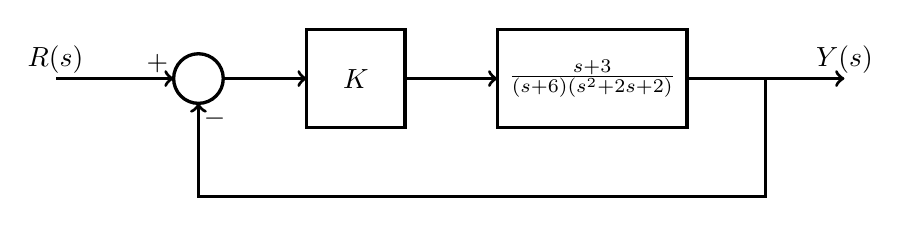
\begin{tikzpicture}[scale=1,inner sep=0pt,outer sep=0pt,very thick,
sysblock/.style={draw,rectangle,inner sep=4pt,minimum width=1.25cm,minimum height=1.25cm,very thick}]

\draw (-2,0) node[draw,circle] (sum1) {$\rule{0pt}{18pt}$};
\draw (0,0) node[sysblock] (K)  {$K$};
\draw (3,0) node[sysblock] (G) {$\frac{s+3}{(s+6)(s^2+2s+2)}$};
\draw[<-] (sum1.180) node[above left=2pt] {$+$} -- ++(-1.5,0) node[above=2pt] {$R(s)$};
\draw[->] (sum1.0) -- (K.180);
\draw[->] (K.0) -- (G.180);
\draw[->] (G.0) --  ++(2,0) node[above=2pt] {$Y(s)$};
\draw[->] (G.0) -- ++(1,0) -- ++(0,-1.5) -| (sum1.-90) node[below right=2pt] {$-$};
\end{tikzpicture}
\end{center}

Which one of the following three root locus plots is (approximately) correct for this closed-loop system as $K$ goes from zero to infinity?  (Hint: you should be able to use your sketching rules to select among the plots, but it's a smart idea to check your answer in Matlab.)

\includegraphics[width=6in]{\mainfolder/LectureNotes/\lecturefolder/HomeworkProblems/Problem04plots.png}
